%%%%%%%%%%%%%%%%%%%%%%%%%%%%%%%%%%%%%%%%%%%%%%%%%%%%%%%%%%%%%%%%%%%%%
%%                                                                 %%
%% Please do not use \input{...} to include other tex files.       %%
%% Submit your LaTeX manuscript as one .tex document.              %%
%%                                                                 %%
%% All additional figures and files should be attached             %%
%% separately and not embedded in the \TeX\ document itself.       %%
%%                                                                 %%
%%%%%%%%%%%%%%%%%%%%%%%%%%%%%%%%%%%%%%%%%%%%%%%%%%%%%%%%%%%%%%%%%%%%%

%%\documentclass[referee,sn-basic]{sn-jnl}% referee option is meant for double line spacing

%%=======================================================%%
%% to print line numbers in the margin use lineno option %%
%%=======================================================%%

%%\documentclass[lineno,sn-basic]{sn-jnl}% Basic Springer Nature Reference Style/Chemistry Reference Style

%%======================================================%%
%% to compile with pdflatex/xelatex use pdflatex option %%
%%======================================================%%

%%\documentclass[pdflatex,sn-basic]{sn-jnl}% Basic Springer Nature Reference Style/Chemistry Reference Style

%%\documentclass[sn-basic]{sn-jnl}% Basic Springer Nature Reference Style/Chemistry Reference Style
\documentclass[pdflatex, sn-mathphys]{sn-jnl}% Math and Physical Sciences Reference Style
%%\documentclass[sn-aps]{sn-jnl}% American Physical Society (APS) Reference Style
%%\documentclass[sn-vancouver]{sn-jnl}% Vancouver Reference Style
%%\documentclass[sn-apa]{sn-jnl}% APA Reference Style
%%\documentclass[sn-chicago]{sn-jnl}% Chicago-based Humanities Reference Style
%%\documentclass[sn-standardnature]{sn-jnl}% Standard Nature Portfolio Reference Style
%%\documentclass[default]{sn-jnl}% Default
%%\documentclass[default,iicol]{sn-jnl}% Default with double column layout

%%%% Standard Packages
%%<additional latex packages if required can be included here>

% The amssymb package provides various useful mathematical symbols
% \usepackage{amssymb}
% The amsthm package provides extended theorem environments
% \usepackage{amsmath}

\usepackage[
    locale=US,
    separate-uncertainty=true,
    per-mode=fraction,    
%    print-unity-mantissa = false, 
]{siunitx}
\DeclareSIUnit\clight{\text{\ensuremath{c}}}
\sisetup{math-micro=\text{µ},text-micro=µ}
\sisetup{detect-weight=true, detect-family=true}

\usepackage{float}
\usepackage{scrhack}
\floatplacement{figure}{htbp}
\floatplacement{table}{htbp}

% % nice tables
\usepackage{booktabs}
\usepackage{multirow}

% reviewing
% \usepackage[textsize=footnotesize]{todonotes}
% \newcommand{\alexander}[1]{\todo[inline,color=green!40]{\textit{Alexander:} #1}}
% \newcommand{\jm}[1]{\todo[inline,color=orange!40]{\textit{Jean-Marco:} #1}}
%%%%

%%%%%=============================================================================%%%%
%%%%  Remarks: This template is provided to aid authors with the preparation
%%%%  of original research articles intended for submission to journals published 
%%%%  by Springer Nature. The guidance has been prepared in partnership with 
%%%%  production teams to conform to Springer Nature technical requirements. 
%%%%  Editorial and presentation requirements differ among journal portfolios and 
%%%%  research disciplines. You may find sections in this template are irrelevant 
%%%%  to your work and are empowered to omit any such section if allowed by the 
%%%%  journal you intend to submit to. The submission guidelines and policies 
%%%%  of the journal take precedence. A detailed User Manual is available in the 
%%%%  template package for technical guidance.
%%%%%=============================================================================%%%%

\jyear{2022}%

%% as per the requirement new theorem styles can be included as shown below
\theoremstyle{thmstyleone}%
\newtheorem{theorem}{Theorem}%  meant for continuous numbers
%%\newtheorem{theorem}{Theorem}[section]% meant for sectionwise numbers
%% optional argument [theorem] produces theorem numbering sequence instead of independent numbers for Proposition
\newtheorem{proposition}[theorem]{Proposition}% 
%%\newtheorem{proposition}{Proposition}% to get separate numbers for theorem and proposition etc.

\theoremstyle{thmstyletwo}%
\newtheorem{example}{Example}%
\newtheorem{remark}{Remark}%

\theoremstyle{thmstylethree}%
\newtheorem{definition}{Definition}%

\raggedbottom
%%\unnumbered% uncomment this for unnumbered level heads

\begin{document}

\title[Muon Deflection]{Simulation of theoretical deflection uncertainty on directional 
muon reconstruction using PROPOSAL}

%%=============================================================%%
%% Prefix	-> \pfx{Dr}
%% GivenName	-> \fnm{Joergen W.}
%% Particle	-> \spfx{van der} -> surname prefix
%% FamilyName	-> \sur{Ploeg}
%% Suffix	-> \sfx{IV}
%% NatureName	-> \tanm{Poet Laureate} -> Title after name
%% Degrees	-> \dgr{MSc, PhD}
%% \author*[1,2]{\pfx{Dr} \fnm{Joergen W.} \spfx{van der} \sur{Ploeg} \sfx{IV} \tanm{Poet Laureate} 
%%                 \dgr{MSc, PhD}}\email{iauthor@gmail.com}
%%=============================================================%%

\author*[1]{\fnm{Pascal} \sur{Gutjahr}}\email{pascal.gutjahr@tu-dortmund.de}

\author[1]{\fnm{Jean-Marco} \sur{Alameddine}}\email{jean-marco.alameddine@tu-dortmund.de}
% \equalcont{These authors contributed equally to this work.}

\author[2]{\fnm{Alexander} \sur{Sandrock}}\email{alexander.sandrock@udo.edu}

\author[1]{\fnm{Jan} \sur{Soedingrekso}}\email{jan.soedingrekso@tu-dortmund.de}

\author[1]{\fnm{Wolfgang} \sur{Rhode}}\email{wolfgang.rhode@tu-dortmund.de}


\affil*[1]{\orgdiv{Dept. of Physics}, \orgname{TU Dortmund University}, \orgaddress{\street{Otto-Hahn-Straße~4}, \city{Dortmund}, \postcode{44227}, \state{NRW}, \country{Germany}}}

\affil[2]{\orgdiv{Faculty of Mathematics and Natural Sciences}, \orgname{Bergische Universität Wuppertal}, \orgaddress{\street{Gaußstraße~20}, \city{Wuppertal}, \postcode{42119}, \state{NRW}, \country{Germany}}}

%%==================================%%
%% sample for unstructured abstract %%
%%==================================%%

\abstract{For uncertainty estimation of reconstruction of the muon direction, the 
deflection of muons along a propagated path in ice and water is simulated using 
the tool PROPOSAL (Propagator with optimal precision and optimized speed for all leptons), which considers multiple scattering and stochastic deflection. 
The deflection per interaction spans several 
orders of magnitude with $\theta \in [\SI{e-9}{\degree},\, \SI{1}{\degree}]$ 
for energies $E < \SI{1}{\peta\electronvolt}$ 
and is rather negligible. The median accumulated 
deflection of a muon with an energy $E_{\mathrm{\mu}} = \SI{500}{\giga\electronvolt}$ 
after a propagated track is about $\theta_{\text{acc}} = 0.10_{-0.02}^{+0.27}\,\si{\degree}$ 
with a $\SI{95}{\percent}$ central interval, 
for propagation distances of $d = 17.5_{-8.0}^{+26.5}\,\si{\kilo\meter}$. 
This is in the order of magnitude of 
the directional resolution of 
present neutrino detectors. The deflection can be simply parametrized in 
dependence of the final muon energy. Furthermore, the deflections are compared to the results 
of the propagation tools MUSIC and GEANT4 and all deflections are in good 
agreement. 
}

\keywords{neutrino astronomy, point-source-analysis, angular resolution}

%%\pacs[JEL Classification]{D8, H51}

%%\pacs[MSC Classification]{35A01, 65L10, 65L12, 65L20, 65L70}

\maketitle

\section{Introduction}\label{sec:introduction}

Neutrinos can cross the universe all the way to earth, since they are 
nearly massless and not charged. On earth, neutrinos can interact 
with a nucleus and produce an electron, muon or tau in the charged current 
via the weak interaction \cite{pdg}. These charged daughter particles are very 
high-energetic and emit Cherenkov light, which can be detected 
by large neutrino telescopes like IceCube \cite{IceCube_Instrumentation} or 
KM3NeT \cite{KM3NeT_Design}. 
By the reconstruction of the direction of the daughter particles, the direction 
of the original neutrino can be inferred. The angular resolution is at its 
best for muons, since they can travel up to a few kilo meters due to their 
large mass, instead of the much lighter electrons and taus - which decay almost 
instantly. Current angular resolutions are 
$\Phi_{\text{I}} > \SI{0.1}{\degree} - \SI{0.3}{\degree}$ for energies 
$E \in [\SI{3}{\tera\electronvolt},\,\SI{3}{\peta\electronvolt}]$ in IceCube 
\cite{IceCube_Resolution2021} 
and 
$\Phi_{\text{K}} < \SI{0.2}{\degree}$ for $E > \SI{10}{\tera\electronvolt}$ in 
KM3NeT/ARCA \cite{KM3NeT_Resolution2021}.
In general, muons do up to several thousand interactions along their propagation, depending 
on their energy, propagation distance and energy cuts, which are mentioned in 
Section~\ref{sec:proposal}.
Since they 
are deflected in each interaction, it is important to study if the accumulated 
deflection along a track impacts the angular resolution of current 
neutrino detectors. 

For this purpose, the lepton propagation 
tool PROPOSAL \cite{koehne2013proposal, dunsch_2018_proposal_improvements} is described in Section~\ref{sec:proposal} first and used to study the muon deflection per interaction in 
Section~\ref{sec:defl_per_int}. Then, the
accumulated deflection is compared to the results of the propagation tools MUSIC and GEANT4 in Section~\ref{sec:accum_defl}. Furthermore, the median deflection is parametrized. The 
paper concludes with a summarized overview in Section~\ref{sec:conclusion}.

\section{Overview of the Simulation Tool PROPOSAL}\label{sec:proposal}

The tool PROPOSAL propagates charged leptons and photons through media und is 
used in this paper to simulate the deflection of muons. For this purpose, 
muons are propagated through the media ice and water 
to estimate the deflection for IceCube and KM3NeT/ARCA. All relevant muon interaction types 
as bremsstrahlung \cite{KKP_1995, Karnaukhov_1999}, photonuclear interaction \cite{Abramowicz_1997} with 
shadowing \cite{ButkevichMikheyev_2002}, electron pair production \cite{epair_kokoulin_petrukhin} with corrections for the 
interaction with atomic electrons \cite{Kelner_1998}, 
ionization by Bethe-Bloch formula with corrections for muons \cite{Rossi} and decay are provided. The interaction processes are sampled by their cross section. Since bremsstrahlung interactions can be 
arbitrary small due to a massless exchange particle, the photon, an energy cut is introduced to avoid an infinite number of bremsstrahlung interactions 
and furthermore to speed up the propagation process. 
The limit is applied with a minimum energy loss
\begin{equation}
    E_{\text{loss,min}} = \min{(E \cdot \texttt{v\_cut}, \texttt{e\_cut})}\,,
\end{equation}
using two parameters - a relative and total energy cut denoted as 
$\texttt{v\_cut}$ and $\texttt{e\_cut}$ with particle energy $E$. The uncertainties are small 
for a relative energy cut $\texttt{v\_cut}\ll 1$, which increases the 
CPU runtime.
A sampled energy loss 
$E_{\text{loss}} < E_{\text{loss,\,min}}$ builds an integrated part of a 
stochastic energy loss referred to as continuous energy loss. The 
propagation process is defined by an initial energy $E_{\text{i}}$ and 
two stopping criteria - a final energy $E_{\text{f,\,min}}$ and a 
maximum propagation distance $d_{\text{min}}$. If the last interaction of 
a propagation is sampled by a stochastic interaction, the true final energy 
$E_{\text{f}}$ can become lower and the 
propagation distance $d$ can be higher than the required limits. 
The deflections for stochastic interactions are parametrized by Van Ginneken 
in \cite{Van_Ginneken} with a direct calculation of the deflection in 
ionization using four-momentum conservation. 
Furthermore, there are parametrizations for deflections given in GEANT4 \cite{GEANT4} 
for bremsstrahlung and photonuclear interaction, which 
are available in PROPOSAL, too.
To estimate the deflection along 
a continuous energy loss, multiple scattering established by Molière 
\cite{moliere_scattering} and the gaussian approximation by Highland 
can be chosen \cite{HIGHLAND_1975}. 
The deflection angle in the plane perpendicular to the muon direction is 
sampled uniformly between $0$ and $2\pi$.
The latest updates with a detailed description of the whole tool can be found 
in \cite{phd_soedingrekso}.
All simulations are done with PROPOSAL $7.3.0$.

\section{Muon deflection per Interaction}\label{sec:defl_per_int}
First, the stochastic deflections introduced by \cite{Van_Ginneken} implemented 
in PROPOSAL are investigated in relation to the two multiple scattering methods. 
For this muons are propagated from $E_{\text{i}} = \SI{1}{\peta\electronvolt}$ to $E_{\text{f,\,min}} = \SI{1}{\tera\electronvolt}$.
The deflections per interaction are presented 
for each interaction type and the total amount in Figure~\ref{fig:defl_per_int}. 
A single deflection 
extend over several orders of magnitude with a median of $\SI{3.9e-6}{\degree}$
and a $\SI{95}{\percent}$ central interval of $[\SI{4.9e-7}{\degree}, \,\SI{1.3e-3}{\degree}]$. 
It follows that the deflections are primarily dominated by multiple scattering, except for a few outliers caused by bremsstrahlung, which 
allows very large energy losses and thus the largest deflections.
The median propagation distance with the lower and upper $\SI{95}{\percent}$ 
interval results to $16.4_{-7.3}^{+24.6}\,\si{\kilo\meter}$.

\begin{figure}
    \centering 
    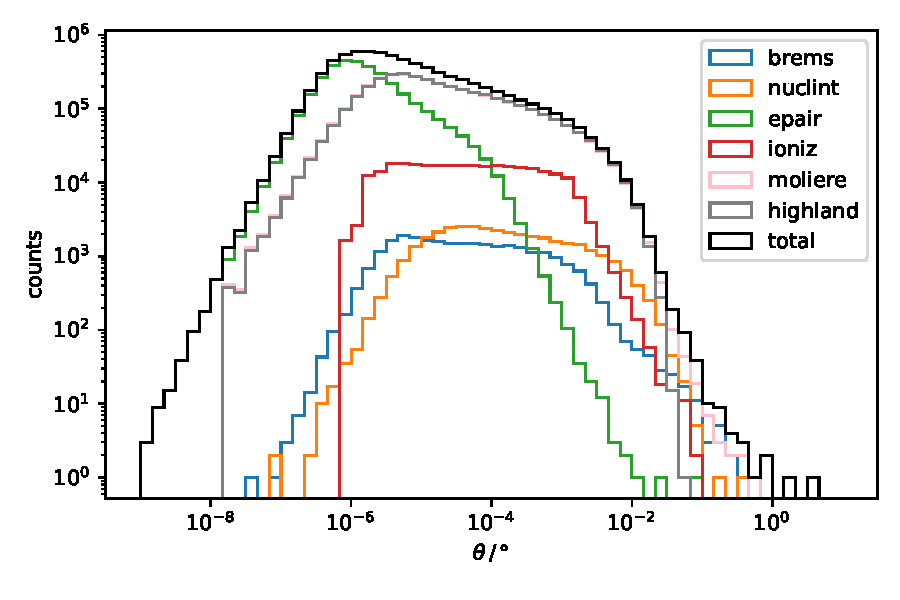
\includegraphics[width=0.8\textwidth]{../../deflection/plots/FINAL/1PeV_1TeV_1000events_deflection_along_sampling.pdf}
    \caption{The deflection $\theta$ per interaction is shown in degree for different mechanisms. The propagation is done for $\num{1000}$ 
    muons from $E_{\text{i}} = \SI{1}{\peta\electronvolt}$ to $E_{\text{f,\,min}} = \SI{1}{\tera\electronvolt}$ using $\texttt{e\_cut} = \SI{500}{\mega\electronvolt}$ and $\texttt{v\_cut} = 0.05$ in ice. Two simulations 
    are done to check both multiple scattering methods Molière and Highland. The total distribution includes all stochastic processes and Molière's. Multiple scattering dominates the deflection. Details are presented in 
    Table~\ref{tab:defl_per_int}.}
    \label{fig:defl_per_int}
\end{figure}

\begin{table}
    \centering 
    \caption{The medians of deflections $\theta$ per interaction from Figure~\ref{fig:defl_per_int} are presented for each interaction type and the total distribution with the upper and lower limits of the $\SI{95}{\percent}$ 
    central content levels.}
    \begin{tabular}{ccccccc}
        \toprule 
        brems & nuclint & epair & ioniz & moliere & highland & total  \vspace{6pt} \\
        $\theta\,/\,\SI{e-5}{\degree}$ & $\theta\,/\,\SI{e-4}{\degree}$ & $\theta\,/\,\SI{e-6}{\degree}$ & $\theta\,/\,\SI{e-5}{\degree}$ & $\theta\,/\,\SI{e-5}{\degree}$ & $\theta\,/\,\SI{e-5}{\degree}$ & $\theta\,/\,\SI{e-6}{\degree}$\\
        \midrule 
        $3.8_{-0.1}^{+297}$ & $1.2_{-0.4}^{+96}$ & $1.3_{-0.2}^{+42}$ & $4.4_{-0.1}^{+181}$& $1.2_{-0.05}^{+222}$ & $1.2_{-0.05}^{+225}$ & $3.9_{-0.2}^{+1285}$\\ 
        \bottomrule
    \end{tabular}
    \label{tab:defl_per_int}
\end{table}

\section{Accumulated Muon Deflection}\label{sec:accum_defl}

As shown in Section~\ref{sec:defl_per_int}, in general the deflection per interaction 
is lower $\sim\SI{1}{\degree}$. Since these deflections accumulate along the 
propagation path, the angle between the incoming muon direction and the outgoing 
muon direction is analyzed. The deflection results as a limit on the 
angular reconstruction accuracy.

At first, the deflections in PROPOSAL are compared to 
the tools MUSIC \cite{MUSIC,comparison_MUSIC_GEANT4_2009} and GEANT4 \cite{GEANT4}.
MUSIC (MUon SImulation Code) is a tool to simulate the propagation of muons 
through media like rock and water considering the same energy losses as in 
PROPOSAL. Also, the losses are divided into continuous and stochastic 
energy losses by a relative energy cut. Several cross-sections, multiple scattering 
methods and parametrizations for stochastic deflection are 
available. For these studies, it is chosen bremsstrahlung \cite{Bremsstrahlung_KKP}, 
nuclear interaction \cite{nulcint_bugaev_Shlepin, bugaev_1980_defl,bugaev_1981_defl} 
and electron pair production \cite{epair_kelner,epair_kokoulin_petrukhin}, 
which deflections are parametrized by \cite{Van_Ginneken}. 
Also, ionization is treated as a stochastic process with the Bethe-Bloch 
formula including knock-on electron production. As scattering, the gaussian 
approximation \cite{HIGHLAND_1975} is set. 
GEANT4 is another common toolkit to simulate the passage of particles through 
a medium with several possibilities and a focus on high-energy 
particle accelerators \cite{GEANT4}. 

A comparison of all three tools is done in Figure~\ref{fig:compare_MUSIC} 
with four different settings in PROPOSAL for the 
accumulated deflection angle $\theta_{\text{acc}}$ and the lateral displacement
$x$. The deflection angles are very similar in all cases. The 
displacement is dominated by GEANT4 and PROPOSAL with Molière scattering, which 
leads to the largest deflections and thus to a larger displacement. 
PROPOSAL with Highland scattering and MUSIC have less outliers, since large 
deflections are neglected in the Gaussian approximation \cite{HIGHLAND_1975}. 
The combination of Highland and \cite{Van_Ginneken} leads to the smallest 
displacement, since in nuclear interaction, the sampling from the root mean squared angle in the 
exponential distribution neglects outliers to larger angles.

Detailed information are given in Table~\ref{tab:compare_MUSIC}. In GEANT4, the 
largest deflections result with $\overline{\theta} = \SI{0.27}{\degree}$ 
and $\overline{x} = \SI{3.3}{\meter}$. The lowest values $\overline{\theta} = \SI{0.22}{\degree}$ and 
$\overline{x} = \SI{2.6}{\meter}$ result in MUSIC. The results of PROPOSAL lay between 
these two tools for all four settings which approves the 
correctness of PROPOSAL.

A measurement of muon deflection in low-$Z$ materials was done in \cite{attwood_2006}. 
From this it can be seen that for $Z < 4$ the scattering angle is overestimated 
by Molière scattering in GEANT4. Hence, the lower scattering in PROPOSAL leads 
to a better precision especially in the region of outliers. The comparison is 
done in liquid $\text{H}_2$ with a thickness of $\SI{109}{\milli\meter}$ and an 
initial particle energy of $E_{\mathrm{i}} = \SI{199}{\mega\electronvolt}$, which 
results via the energy-momentum relation of an in \cite{attwood_2006} used beam momentum 
of $p = \SI[per-mode=symbol]{168.9}{\mega\electronvolt\per\clight}$. 
The result is presented in Figure~\ref{fig:attwood_comparison}.
\begin{figure}
    \centering 
    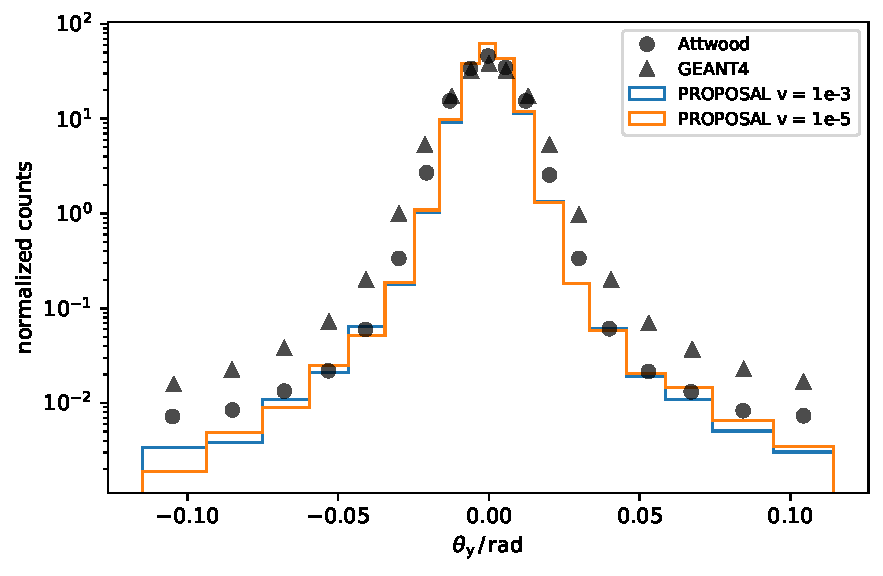
\includegraphics[width=0.8\textwidth]{../../deflection/plots/FINAL/attwood_comparison_moliere_E199MeV_final.pdf}
    \caption{In total $\num{e5}$ muons with $E_{\mathrm{i}} = \SI{199}{\mega\electronvolt}$ are propagated through 
    $\SI{109}{\milli\meter}$ of liquid $\text{H}_2$. In PROPOSAL, the simulation is done 
    for two different energy cuts $\texttt{v\_cut} = \num{e-3}$ and $\texttt{v\_cut} = \num{e-5}$ using Molière scattering.
    Measured data of Attwood and simulation data of GEANT4 are taken from \cite{attwood_2006}. The figure presents 
    the normalized counts in dependence of the projected scattering angle $\theta_{\mathrm{y}}$ in radians. At small deflections, PROPOSAL 
    is underestimating, but at larger deflections the result seems to be more accurate than GEANT4's.}
    \label{fig:attwood_comparison}
\end{figure}

\begin{figure}
    \centering 
    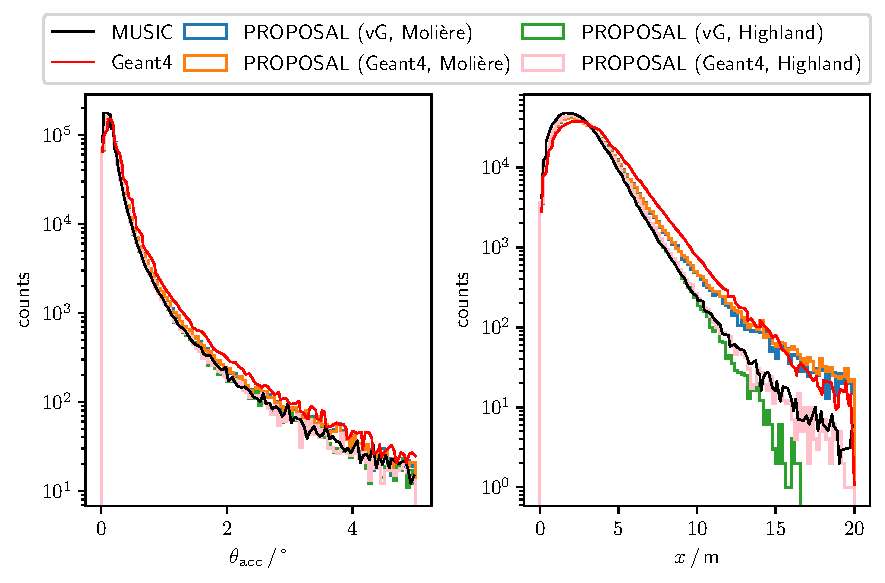
\includegraphics[width=0.98\textwidth]{../../deflection/plots/FINAL/2TeV_1e6events_accumulated_defl_paper_combined.pdf}
    \caption{A comparison of the results of MUSIC, GEANT4 and PROPOSAL is presented for $\num{1000000}$ negative charged muons propagated with 
    $E_{\text{i}} = \SI{2}{\tera\electronvolt}$ over a distance of 
    $\SI{3}{\kilo\meter}$ in water. A $\texttt{v\_cut} = 0.001$ is set. In PROPOSAL, 
    bremsstrahlung and photonuclear interaction are parametrized by 
    Van Ginneken (vG) and GEANT4 and both scattering methods are checked. 
    Left: The accumulated deflection $\theta_{\mathrm{acc}}$ in degree is very similar in all cases.
    Right: The lateral displacement $x$ in meter depends 
    on the scattering method. Molière scattering leads to larger distances.
    Detailed information are given in 
    Table~\ref{tab:compare_MUSIC}. The results for MUSIC and GEANT4 are taken from 
    \cite{comparison_MUSIC_GEANT4_2009}.}
    \label{fig:compare_MUSIC}
\end{figure}

\begin{table}
    \small
    \centering
    \caption{The survival probability $p_{\text{s}}$ - otherwise the muon decays before, the mean survived muon 
    energy $\overline{E}_{\text{f}}$, the mean scattered angle $\overline{\theta}$ 
    and the mean displacement $\overline{x}$ are presented for all cases from 
    Figure~\ref{fig:compare_MUSIC}. For all means, the standard deviation is given.
    The largest deflection and displacement result in the tool GEANT4, which has the lowest mean survived energy. The lower the energy, the larger the deflection.}
    \begin{tabular}{l|cc|cccc}
        \toprule
        & & & \multicolumn{4}{c}{PROPOSAL} \\
        &  & & \multicolumn{2}{c}{Molière} & \multicolumn{2}{c}{Highland} \\
        & MUSIC & GEANT4 & vG & GEANT4 & vG & GEANT4 \\
        \midrule
        $p_{\text{s}}\,/\,\si{\percent}$ & 77.9 & 79.3 &  \multicolumn{4}{c}{77.9}\\
        $\overline{E}_{\text{f}}\,/\,\si{\giga\electronvolt}$ & 323 & 317 & \multicolumn{4}{c}{331$\pm$178} \\
        $\overline{\theta}\,/\,\si{\degree}$ & 0.22 & 0.27 & 0.24$\pm$0.45 & 0.24$\pm$0.45 & 0.22$\pm$0.35 & 0.22$\pm$0.35   \\
        $\overline{x}\,/\,\si{\meter}$ & 2.6 & 3.3 & 2.9$\pm$2.6 & 2.9$\pm$2.6 & 2.7$\pm$1.6 & 2.7$\pm$1.7  \\
     \bottomrule
    \end{tabular}
    \label{tab:compare_MUSIC}
\end{table}

For current analyses, it is important to study the impact of the muon 
deflection on the angular resolution to estimate an uncertainty on the reconstruction.
For this purpose, four different initial energies 
from $E_{\text{i}} = \SI{10}{\tera\electronvolt}$ to 
$E_{\text{i}} = \SI{10}{\peta\electronvolt}$ are used and the final 
energy is set to $E_{\text{f,\,min}} \geq \SI{10}{\giga\electronvolt}$ with 
$E_{\text{f,\,min}} < E_{\text{i}}$ for each simulation. To compare the results of 
a total of $\num{36}$ simulations, the median of the deflection distribution 
with a $\SI{95}{\percent}$ central interval is presented in 
Figure~\ref{fig:fit_median}.
The lower the final muon energy, the larger the accumulated deflection. 
For energies $E_{\text{f}} = \SI{1}{\peta\electronvolt}$, the median deflection 
is lower than $\SI{e-3}{\degree}$. For energies $E_{\text{f}} = \SI{10}{\giga\electronvolt}$, 
angles larger than $\SI{1}{\degree}$ are possible. For energies  
$E_{\text{f}} \approx \SI{100}{\giga\electronvolt}$, 
there is a small overlap of the deflection with the angular resolution of KM3NeT 
\cite{KM3NeT_Resolution2016}. The resolution of IceCube is a bit worse and 
therefore not affected \cite{IceCube_Resolution2021}. 
The kinematic angle between the incident neutrino and the produced muon is 
larger than the deflection in the presented region from $\SI{300}{\giga\electronvolt}$
to $\SI{200}{\tera\electronvolt}$. Here it must be noted that the kinematic angle 
and the resolution of ARCA are presented in dependence of the neutrino energy 
in \cite{KM3NeT_Resolution2016, KM3NeT_Resolution2021}. Hence, a rescale to 
the muon energy is done using the energy transfer of the neutrino to 
the nucleus \cite{GANDHI199681}. This shifts both the curves to lower energies. 
Since all of these simulations are done 
in ice, the same simulations are done in water. The deviations of the medians
are less than $\SI{1}{\percent}$ for all energies.

Furthermore, in Figure~\ref{fig:fit_median} there are only $12$ medians visible, 
instead of $36$ which is the total amount of all simulations. This result points 
out that the total deflection of a muon 
primarily depends on the final muon energy.
The initial muon energy is negligible. 
Hence, the reconstructed muon 
energy in a detector can be used to estimate a theoretical deflection. For this 
purpose, the following fit-function 
\begin{equation}
     f(x) = a \cdot x^3 + b \cdot x^2 + c \cdot x + d \,,
    \label{eqn:fit_median}
\end{equation}
can be applied with the parameters 
\begin{align}
    a =& +0.024 \pm 0.001\,,  & c =& +0.379 \pm 0.057\,,\\
    b =& -0.312 \pm 0.016\,,  & d =& -0.216 \pm 0.058\,,
\end{align}
in the logarithmic space via 
\begin{align}
    g(x) =& 10^{f(x)}\,, & x =& \log_{10}\left(\frac{E_{\text{f}}}{\si{\giga\electronvolt}}\right)\,.
\end{align}

\begin{figure}
    \centering 
    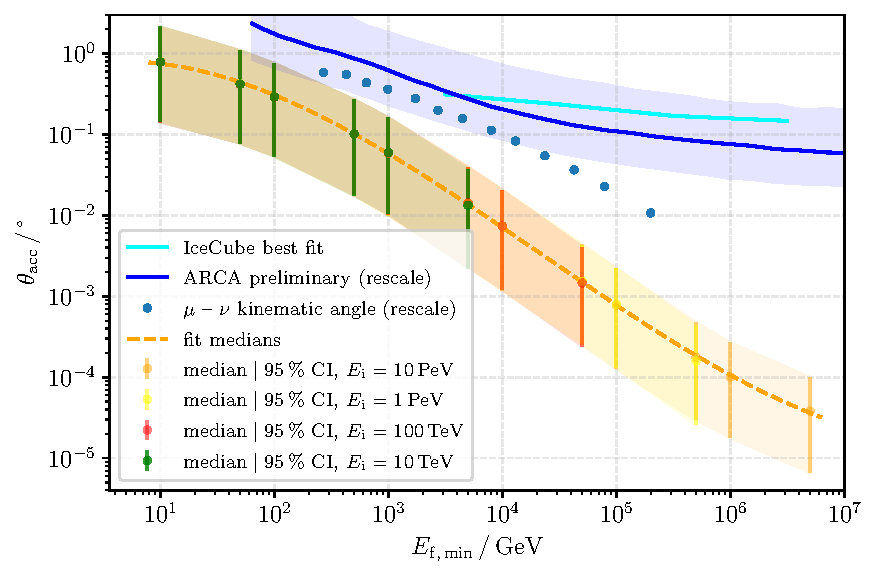
\includegraphics[width=0.96\textwidth]{../../deflection/plots/FINAL/fit_median_defl_cut_10percent_only_poly_new_resolution_rescale_no_icecube_paper_final.pdf}
    \caption{The median of the accumulated deflection $\theta_{\text{acc}}$ in degree 
    with a $\SI{95}{\percent}$ 
    central interval is shown for four different initial energies $E_{\text{i}}$. 
    Each data set includes more than $\num{50000}$ events with the requirement 
    that the true final particle energy $E_{\text{f}}$ is maximum 
    $\SI{10}{\percent}$ below the set final energy $E_{\text{f,\,min}}$,   
    $E_{\text{f}} > E_{\text{f,\,min}} \cdot 0.9$. The energy cuts are $\texttt{e\_cut} = \SI{500}{\mega\electronvolt}$ and $\texttt{v\_cut} = 0.05$ and 
    Molière scattering is chosen. Simulations are done in ice, the deviation 
    of the medians in a water based simulation are less than $\SI{1}{\percent}$.
    Since the medians overlap for different initial energies, there is no 
    strong impact of the initial energy on the median deflection. These 
    medians can be fit by a third degree polynomial in the log-space as 
    shown in Equation~\eqref{eqn:fit_median}. The kinematic angle between the muon and 
    neutrino is taken from \cite{KM3NeT_Resolution2016}. Since the kinematic angle and 
    the angular resolution of ARCA taken from \cite{KM3NeT_Resolution2016, KM3NeT_Resolution2021} are 
    presented in dependence of the neutrino energy, a rescale to the muon energy is done 
    using the energy transfer to the nucleus \cite{GANDHI199681}. 
    For energies 
    $E_{\text{f}} \approx \SI{100}{\giga\electronvolt}$, there is a minimal influence of deflection on the angular resolution of 
    KM3NeT/ARCA \cite{KM3NeT_Resolution2021}. The resolution shown by IceCube is not 
    impacted \cite{IceCube_Resolution2021}.}
    \label{fig:fit_median}
\end{figure}

\section{Conclusion}\label{sec:conclusion}

At first, the recently into PROPOSAL implemented stochastic deflection is 
used to study the muon deflection per interaction. Mainly, the deflection 
is dominated by multiple scattering except for a few stochastic 
outliers by bremsstrahlung. These angles are lower $\sim\SI{1}{\degree}$. 

The results of PROPOSAL are tested against the common tools MUSIC and 
GEANT4 and all are in good agreement. In low-$Z$ materials, the region of outlier 
deflections is described better with PROPOSAL than GEANT4.

The median accumulated deflection depends on the final muon energy, primarily. 
The outcome is fit by a polynom and can be used for 
a theoretical estimation of the muon deflection in water and ice.
This final energy can be interpreted as the muon energy at detector entry 
in neutrino telescopes. 
The result can 
be used to estimate the muon deflection before the detector entry.
Hence, this deflection defines a lower limit on the directional resolution.
At energies of $\SI{100}{\giga\electronvolt}$, there is a small impact of the muon deflection on the angular 
resolution of KM3NeT.


\backmatter

\bmhead{Acknowledgments}

MISSING


% \begin{appendices}

% \section{Section title of first appendix}\label{secA1}

% An appendix contains supplementary information that is not an essential part of the text itself but which may be helpful in providing a more comprehensive understanding of the research problem or it is information that is too cumbersome to be included in the body of the paper.

%%=============================================%%
%% For submissions to Nature Portfolio Journals %%
%% please use the heading ``Extended Data''.   %%
%%=============================================%%

%%=============================================================%%
%% Sample for another appendix section			       %%
%%=============================================================%%

%% \section{Example of another appendix section}\label{secA2}%
%% Appendices may be used for helpful, supporting or essential material that would otherwise 
%% clutter, break up or be distracting to the text. Appendices can consist of sections, figures, 
%% tables and equations etc.

% \end{appendices}

%%===========================================================================================%%
%% If you are submitting to one of the Nature Portfolio journals, using the eJP submission   %%
%% system, please include the references within the manuscript file itself. You may do this  %%
%% by copying the reference list from your .bbl file, paste it into the main manuscript .tex %%
%% file, and delete the associated \verb+\bibliography+ commands.                            %%
%%===========================================================================================%%

%% BioMed_Central_Bib_Style_v1.01
    

\bibliography{lit}% common bib file
% \bibliography{sn-bibliography}% common bib file
%% if required, the content of .bbl file can be included here once bbl is generated
%%\input sn-article.bbl

%% Default %%
%%\input sn-sample-bib.tex%

\end{document}
